%\documentclass[journal=jpccck,manuscript=article]{achemso}
%\usepackage[numbers,super]{natbib}
%
%\usepackage{graphicx}
%\usepackage{xcolor}
%\usepackage{todonotes}
%
%\def\ket#1{| #1 \rangle}
%\def\bra#1{\langle #1 |}
%
%\usepackage[utf8]{inputenc} % set input encoding (not needed with XeLaTeX)
%\usepackage{verbatim}
%\usepackage{amsfonts}
%\usepackage{graphicx}
%\newcommand{\overbar}[1]{\mkern 2.2mu\overline{\mkern-2.2mu#1\mkern-2.2mu}\mkern 2.2mu}
%\usepackage{multirow}
%\usepackage{array}
%\usepackage{varwidth}
%\usepackage{bm}
%
%\title{Pair Natural Orbitals ++ approach for Coupled Cluster Linear-Response Theory}
%\author{Ashutosh Kumar}
%\affiliation{Department of Chemistry, Virginia Tech, Blacksburg, Virginia 24061, U.S.A.}
%\author{T.\ Daniel Crawford}
%\email{crawdad@vt.edu}
%\affiliation{Department of Chemistry, Virginia Tech, Blacksburg, Virginia 24061, U.S.A.}
%
%\date{\today}
%
%\begin{document}
%
%\begin{abstract} We present here the the modified  pair natural-orbital (NO) 
%approach, which we call PNO++ for a compact representation of the 
%response of the coupled cluster wavefunction to external electric
%and magnectic fields. In our earlier work,%\cite{McAlexander15}
%we showed that the regular PNO method performs rather poorly for 
%%The frozen-virtual natural-orbital (NO) approach, whereby the
%%unoccupied-orbital space is constructed using a correlated density such as
%%that from many-body perturbation theory, has proven to yield compact wave
%%functions for determining ground-state correlation energies and associated
%%properties, with corresponding occupation numbers providing a guide to the
%%truncation of the virtual space.  In this work this approach is tested for the
%%first time for the calculation of higher-order response properties,
%%particularly frequency-dependent dipole polarizabilities using coupled-cluster
%%theory.  We find that such properties are much more sensitive to the
%%truncation of virtual space in the natural orbital (NO) basis than in the
%%original canonical molecular orbital (CMO) basis, with truncation errors
%%increasing linearly with respect to the number of frozen virtual NOs.  The
%%reasons behind this poor performance include the more diffuse nature of NOs
%%with low occupation numbers as well as the reduction in sparsity of the
%%perturbed singles amplitudes in the NO basis and the neglect of orbital
%%response.  We tested a number of approaches
%%to improve the performance of the NO space, including the use of a
%%field-perturbed density to define the virtual orbitals and various
%%external-space corrections.  The truncation of the CMO space, on the other
%%hand, yields errors in coupled-cluster dipole polarizabilities of less than
%%2\% even after removing as much as 50\% of the full virtual space. We find
%%that this positive performance of the CMO space results from a cancellation of
%%errors due to the truncation of the unperturbed and perturbed amplitudes, as
%%well as sparsity of the singles amplitudes.  We introduce a simple criterion
%%called a dipole amplitude to use as a threshold for truncating the CMO basis
%%for such property calculations.  \end{abstract}
%\end{abstract}
%\maketitle

\section{Introduction}
Accurate {\em ab initio} models like the coupled cluster theory have been used quite reliably to 
predict the chiroptical properties of molecules. However, they have been limited to very 
small system sizes due to the heavy computational expenses associated with such methods. 
For example, the coupled cluster singles and doubles method (CCSD) has a high polynomial scaling of 
$O(N^6)$, where N is some measure of the system size. This is clearly unphysical as the phenomenon 
of dynamic electron-correlation, which these methods aim to capture, is local in nature.\cite{Saebo86} This 
steep scaling can be attributed to the use of delocalized canonical Hartree-Fock MOs (CMOs) as the one 
electron basis for representing the wavefunction. Local correlation techniques try to exploit the intrinsic 
sparsity in correlated wavefunctions by unitarily localizing the occupied orbitals (LMOs) using methods 
like Boys-Foster, Pipek-Mezey\cite{BoughtonPulay93} etc. and constructing excitation domains corresponding to each LMO. 
The sizes of these domains are usually very small compared to the full virtual space and become constant 
in the asymptotic limit, making these approaches reduced-scaling. Saebo and Pulay's introduction of projected 
atomic orbitals (PAO) as a representation of the virtual space stands as one of the earliest works in this 
regard\cite{Saebo86,Pulay83,PulaySaebo93}. As the name suggests, PAOs are formed by projecting out the occupied MO components from the 
AO basis. Since the PAOs are centered on atoms (just like AOs), an excitation domain for a given LMO can 
be constructed by including only those PAOs which are on or near the atoms associated with that LMO. 
Subsequently, domains corresponding to a pair of LMOs can be formed by taking a union of the PAO space of both 
the LMOs and so on. Werner, Sch{\"u}tz and co-workers \cite{Schutz00a,Schutz00b,Schutz01} were the first to apply these concepts within 
the framework of CC theory. By employing truncated PAO domains coupled with other approximations like weak 
and distant pairs, they were able to achieve linear scaling while maintaining accurate description of 
ground-state properties like reaction enthalpies, thermodynamic constants etc.\cite{Hampel96, Schutz00a,Schutz00b,Schutz01,Saebo86,Pulay83,PulaySaebo93}. Crawford and King 
were the first to use PAOs with the equation of motion CCSD method to calculate excitation energies\cite{CrawfordKing02}. 
In a similar work, Korona and Werner\cite{Korona04} constructed state specific PAO domains to minimize the average 
localization errors for their test set to only 0.06 ev. Schutz and co-workers extended this approach with 
density-fitted second order coupled cluster (CC2) \cite{Christiansen95:CC2} method to calculate excited state properties of 
large systems.\cite{Schutz03} However, these approaches could require very large domian sizes depending on the 
character of the excited state, for example, excitations in a charge-transfer excited state could be 
fairly non-local. PAOs have also been used within the context of CC linear response theory to calculate 
higher-order response properties like (hyper)polarizabilities, chiroptical response etc. albeit on a 
much smaller scale. In 2004, Korona and Werner\cite{Korona04} used PAOs with local coupled cluster singles 
and doubles method (LCCSD) to calculate electric dipole moments and static polarizabilities where they got 
average errors of 1.61\% and 0.48\% respectively. Further minimization of the errors required building bigger 
domains leading to a significant increase in computational expenses. In the same year, Russ and Crawford\cite{Russ04} 
used a modified domain building procedure within the PAO framework, where they augmented the ground state 
orbital domains on the basis of first-order orbital response coefficients obtained by sloving the coupled-perturbed 
Hartree-Fock equations, to calculate CC static polarizabilities. A few years later, they extended this 
formalism to calculate dynamic polarizabilities and optical rotations\cite{Russ08}. While the localization errors 
for linear molecular structures were shown to be only a few percent of canonical results, three dimensional 
compounds required very large domains, especially for optical rotations. A similar conclusion was drawn 
when Friedrich and co-workers applied the incremental scheme, a fragmentation based local correlation technique 
to calculate CC dynamic polarizabilities.\cite{Friedrich15} For a more detailed overview of the applications of PAO based 
methods in this field, please refer to ref\cite{McAlexander15:LRCC}. Within the framework of local correlation, 
the pair natural orbitals (PNOs) introduced in 1970s by Edimnston and Krauss\cite{Edmiston66}, Meyer\cite{Meyer73}, Ahlrichs, 
Kutzelnigg, Staemmler and co-workers\cite{Ahlrichs75} and orbital specific virtuals (OSVs) developed by Chan and 
co-workers in 2011 \cite{Yang12}, are other popular alternatives to PAOs for a compact representation of the virtual 
space. In the local PNO (LPNO) approach, each pair of LMOs have their own virtual space which can be obtained 
by the diagonalization of the virtual-virtual block of an approximate 1-electron pair specific density. 
The OSV approach on the other hand involves diagonalization of a separate density for each LMO. Even though 
the PNOs were shown be to be quite useful as a wavefunction compression technique, they were initially 
abandoned due to the computational costs involved in the transformation of the two electron 
integrals, onlyto be revived later by Neese and co-workers in 2008 by making use of the density-fitting procedure
\cite{Neese09,NeeseCCSD09}. They also proposed a variant of the LPNO approach, a scheme which they call domain based LPNO (DLPNO), 
where the PNOs are expressed in terms of PAOs, to achieve near-linear scaling behavior in MP2 and CC calculations
\cite{Riplinger16}. Following their pioneering works, the LPNO and the DLPNO methods has been used quite sucessfully to study 
ground state properties of molecular systems previously unreachable by canonical correlated methods. 
H{\"a}ttig and co-workers were the first to extend this scheme to excited states by using state-specific 
PNOs generated from CIS(D) densities at CC2 level of theory\cite{Hattig13} and recently with CCSD.\cite{Hattig18}. Valeev and 
co-workers\cite{Chong18} recently implemented a state-averaged L-PNO-CCSD simulation program by taking an average of the 
CIS(D) densities over a desired set of excited states. Similar works employing state-specific natural 
transition orbitals and natural orbitals for calculating excitation energies have also been reported\cite{Mester17,Mester18,Baudin17,HofenerKlopper17}. Our group implemented the LPNO scheme in conjunction with CC2 and CCSD linear response (LR) theory  
to calculate dynamic polarizabilities and specific rotations of different chiral molecules ranging from linear
(H2)n helices to cagelike 1r-4r-norbornenone, where consistent with earlier studies, PNOs were found
to be much more compact than the PAOs and OSVs for representing the wavefunction. However, the truncation errors 
in specific rotations for 3-dimensional structures were quite large and the convergence of both the properties 
towards the canonical result turned out to be very slow\cite{McAlexander15:LRCC}. The failure of the regular LPNO-CC2/CCSD-LR approach
for higher-order response properties could be attributed to the inability of the ground-state MP2 density to 
capture the response of the wavefunction, as shown in our earlier work with natural orbitals (NOs)\cite{Kumar17}. However,
we have recently demonstrated that the NOs obtained from ``perturbation aware" densities are better suited
for calculating these response properties.\cite{Kumar18:1} In this paper, we extend this approach which we have named 
PNO++ by constructing second-order pair specific perturbed densities, and compare its performance with 
the regular method for the same test systems as our earlier PNO paper.
\section{Theory}
\subsection{Coupled Cluster Response Theory}
Coupled cluster (CC) response theory has been proven to be quite a reliable and accurate theoretical
tool to calculate higher-order response properties. Within this formalism,
one expands the time-dependent expectation value of a time-independent operator 
in different orders of the perturbation. The response functions can then be identified 
as fourier transforms (FT) of the time-dependent expansion terms up to a given order, ex. the
linear response function (LRF) is the FT of terms appearing in the first order in the
expansion. CC-LRF for time independent operators $A$ and $B$ can be written as,
\\
\begin{equation}
{\langle\langle A;B\rangle\rangle}_{\omega_1} =  \frac{1}{2}\hat{P}(A,B)[\langle 0 | \
[\hat{Y}^{B}_{\omega_1}, \bar{A}]|0\rangle + \langle 0 | \
(1 + \hat{\Lambda})|[\bar{A},\hat{X}^{B}_{\omega_1}]|0\rangle]
\end{equation}
\\
where $\hat{P}(A,B)$ is a symmetrizing operator which simultaneously interchanges 
operators $A$ and $B$ and takes the complex conjugate of the expression, $\omega_1$ 
is the frequency of the external field, $|0\rangle$ is the reference wavefunction, $\hat{\Lambda}$ is
a linear de-excitation operator that parametrizes the CC left hand wavefunction, 
overbar on operator $A$ denotes a similarity transformation with the ground state 
$T$ operator, $\bar{A} = e^{-\hat{T}}\hat{A}e^{\hat{T}}$ and $\hat{X}^{B}_{\omega_1}$ 
and $\hat{Y}^{B}_{\omega_1}$ are the first-order right and left hand perturbed 
amplitudes corresponding to perturbation operator $B$ respectively.
The LRF expression above can be re-written in terms of frequency-dependent first-order 
perturbed densities ${D^{B^{\omega_1}}_{pq}}^{(1)}$, 
\\
\begin{equation}
\begin{split}
{\langle\langle A;B\rangle\rangle}_{\omega_1} & =  \frac{1}{2}\hat{P}(A,B)[\sum_{pq}A_{pq}\langle 0 | \
\hat{Y}^{B}_{\omega_1}, \overbar{a^{\dagger}_{p}a_q}]|0\rangle + \langle 0 | \
(1 + \hat{\Lambda})|[\overbar{a^{\dagger}_{p}a_q},\hat{X}^{B}_{\omega_1}]|0\rangle] \\
& = \frac{1}{2}\hat{P}(A,B) \big[\sum_{pq} A_{pq}[{D^{B^{\omega_1}}_{pq}}]^{(1)}\big]
\end{split}
\end{equation}
\\
where $a^{\dagger}_{p}$ and $a_q$ are creation and annihilation operators respectively. 
In spin orbitals, the virtual-virtual block of this density looks like,
\\
\begin{equation}
{D^{B^{\omega_1}}_{ab}}^{(1)}= \frac{1}{2}\sum_{ijc}[\lambda^{ij}_{ac}X^{bc}_{ij} \
+ Y^{ij}_{ac}t^{bc}_{ij}] + \sum_i[\lambda^{i}_{a}X^{b}_{i}\
+ Y^{i}_{a}t^{b}_{i}] 
\end{equation}
\\
where $X$ and $Y$ are the right and left hand first order perturbed amplitudes associated with 
perturbation $B$ at frequency $\omega_1$. These amplitudes can be obtained 
by solving a linear system of equations,  
\\
\begin{equation}
\begin{split}
& \sum_\nu{(\bar{H} - \omega I)}_{\mu\nu}X_{\nu}^{B} = -\bar{B}_{\mu} \\
&\sum_\nu Y_{\nu}^{B}{(\bar{H} + \omega I)}_{\nu\mu}
= -  \sum_\nu X_{\nu}^{B} F^{'}_{\nu\mu} - \bar{B}^{'}_{\mu}
\end{split}
\end{equation}
where,
\begin{equation}
\begin{split}
&{(\bar{H} \pm \omega I)}_{\mu\nu} = \langle \mu | \big[(\bar{H} \pm \omega I),\tau_\nu\big] |0\rangle\\
&F^{'}_{\nu\mu} = \langle 0|(1 + \hat{\Lambda})|\big[\big[\bar{H},\tau_\nu\big],\tau_\mu\big] |0 \rangle\\ 
&\bar{B}_{\mu} = \langle \mu|\bar{B}|0 \rangle \\
& \bar{B}^{'}_{\mu} = \langle 0|(1 + \hat{\Lambda})|\big[\bar{B},\tau_\mu\big] |0 \rangle.
\end{split}
\end{equation}
Here $\tau_\mu$, $\tau_\nu$ are operators which generate excited determinats $|\mu\rangle$
and $|\nu\rangle$ by acting on the reference wavefunction $|0\rangle$. Once, we solve for 
$X_{\nu}^{B}$ and $Y_{\nu}^{B}$ amplitudes, the first-order perturbed density can be built 
from eq.(5.3) to construct the CC-LRF. Elements of the dynamic polarizability ($\bm{\alpha}$) 
and optical rotation ($\bm{\beta}$) tensors can be obtained from the LRF with appropriate 
perturbation operators. For example,
\begin{equation}
\begin{split}
& \alpha_{xy}(\omega) = {\langle\langle \mu_x;\mu_y\rangle\rangle}_{\omega_1}\\
&\beta_{xy}(\omega) = {-\text{Im} \langle\langle \mu_x;m_y\rangle\rangle}_{\omega_1} \\
\end{split}
\end{equation}
where $\bm{\mu} = \sum_i q_i \bm{r_i} $, $\bm{m} = \sum_i \frac{q_i}{2m_i} \bm{r_i} \times \bm{p_i}$
and ``Im" signifies that $\beta_{xy}(\omega)$ equals the imaginary part of the corresponding LRF.
\subsection{Ground State PNOs}
The first step in any local correlation approach is the induction of sparsity in the
occupied space. Standard techniques like Boys-Foster, Pipek-Mezey\cite{BoughtonPulay93} accomplish this by 
producing localized MOs or LMOs. The PNOs for a given pair of LMOs $ij$ can then be 
defined by a unitary rotation of the virtual orbitals,
\begin{equation}
|\bm{\bar{a}}^{ij}\rangle = \sum_a |a\rangle \bm{Q}^{ij}_{a\bar{a}}
\end{equation}
where the transformation matrix $\bm{Q}^{ij}_{a\bar{a}}$ is the eigenvector
of the pair $ij$'s contribution to the virtual-virtual block of the one
electron density matrix (1-RDM) i.e $\bm{D} = \sum\limits_{ij}[\bm{D}^{ij}]$.
\begin{equation}
\bm{D}^{ij} \bm{Q}^{ij} = \bm{Q}^{ij} \bm{n}^{ij}
\end{equation} 
The eigenvalues $\bm{n}^{ij}$ are referred to as ``occupation numbers" (ONs) and 
can be seen as a metric for estimating the importance of the corresponding PNO
for describing electron correlation effects for the pair $ij$. For CCSD/CC2 
ground state calculations, approximate pair densities are usually formed from 
the MP2 amplitudes,
\begin{equation}
\bm{D}^{ij} = \frac{2}{1+\delta_{ij}} (\bm{T}^{ij}\tilde{\bm{T}}^{ij\dagger} + \bm{T}^{ij\dagger}\tilde{\bm{T}}^{ij})
\end{equation}
where, 
\begin{equation}
\begin{split}
\tilde{\bm{T}}^{ij} = 2\bm{T}^{ij} - \bm{T}^{ij\dagger} \\
T^{ij}_{ab} = \frac{\langle ab|ij \rangle}{f_{ii} + f_{jj} - \epsilon_a - \epsilon_b}.\\
\end{split}
\end{equation} 
\\
Here, indices $i,j,k$ and $a,b,c$ have been used for occupied and virtual orbitals respectively. The 
integrals $\langle ab|ij \rangle$ are in physicist notation, $f_{ii}$ and $f_{jj}$ are the
$i^{th}$ and $j^{th}$ diagonal elements of the Fock matrix in the LMO basis and 
$\epsilon_a$, $\epsilon_b$ are the orbital energies of the canonical virtual orbitals
$a$ and $b$ respectively. The PNOs with ONs smaller than a given threshold (usually
in $10^{-6} - 10^{-8}$ range) are then neglected as they have minimal contributions
to the total correlation energy. Finally, the canonical CC2/CCSD equations are reformulated
or refactored in terms of these truncated PNO transformations. It should be noted that the virtual
spaces of different pairs of LMOs are non-orthogonal to each other due to which the transformation
of amplitudes from one pair to another requires a overlap metric given by, 
\begin{equation}
%\bm{S}^{ij,kl}_{\bar{a}_{ij},\bar{a}_{kl}} = {\bm{Q}^{ij}_{a,\bar{a}_{ij}}}^{\dagger} {\bm{Q}^{kl}_{a,\bar{a}_{kl}}}
\bm{S}^{ij,kl} = {\bm{Q}^{ij}}^{\dagger} \bm{Q}^{kl}
\end{equation}
\subsection{Perturbed PNOs}
It was shown from our earlier work that the regular LPNO-[CCSD/CC2]-LR approach has
very slow convergence towards the full canonical result both for dynamic polarizabilities
and specific rotations. This is unsurprising since the sparsity of perturbed 
and unperturbed amplitudes are usually very different from each other. Thus, the 
pair densities should be able to capture the response of the ground state amplitudes. 
Recent reduced scaling works on EOM-CC2/CCSD excitation energies employ 
PNO-MP2 and PNO-CIS(D) densities for ground and excited state calculations respectively.\cite{Hattig13,Hattig18}
However, for caluclating response properties using CC-LR theory, one needs to express both 
unperturbed and perturbed amplitudes in the same PNO basis in order to match the results
obtained from finite field procedures. Due to this constraint, two different 
schemes could be explored where a) PNOs are defined from perturbed densities b) effective PNOs 
are obtained by a union of truncated PNOs defined from MP2 and perturbed densities. It should
be noted that one can't just add ground state and perturbed densities together to define an effective
density as they are not in the same units. We have implemented scheme a) in this work and call it LPNO++.
This approach can be justified due to the fact that our target is not total energies but the 
derivative of the total energies in the presence of external fields. Furthermore, it can
be shown that on replacing the CC ground state amplitudes with that of MP2 in CC-LR theory
one introduces minimal errors for both polarizabilities and specific rotations.\cite{Kumar18:2} 
Hence, even though LPNO++ can't be expected to work as well as LPNO for ground state 
calculations, it can capture the response of the wavefunction very efficiently and 
hence should perform a lot better for these kinds of properties. The LPNO++ approach
involves creation of a perturbation specific density for each $ij$ pair. 
This is an extension of our work on natural orbitals where we showed that second-order
perturbed densities can be used quite efficiently for calculating response properties\cite{Kumar18:1}.
For a given perturbation A, the LPNO++ density is constructed by replacing the MP2 
$T^{ij}_{ab}$ amplitudes by the corresponding perturbed amplitudes $X^{ij}_{ab}$.
\begin{equation}
\bm{D}^{A;ij} = \frac{2}{1+\delta_{ij}} (\bm{X}^{ij}\bm{\tilde{X}}^{ij\dagger} + \bm{X}^{ij\dagger}\bm{\tilde{X}}^{ij})
\end{equation}
Rewriting the first part of eq.(5.4),
\begin{equation}
X_{\mu}^{A} = -\sum_{\nu}{{(\bar{H} - \omega I)}^{-1}}_{\mu\nu}\bar{A}_{\nu}
\end{equation}
one can see that an obvious guess for $X^{ij}_{ab}$ amplitudes could be constructed as
\begin{equation}
X^{ij}_{ab} =  \frac{\bar{A}^{ij}_{ab}}{f_{ii} + f_{jj} - \epsilon_a - \epsilon_b} 
\end{equation} 
since the leading contribution to the inverse of the diagonally dominant $(\bar{H} - \omega I)$ matrix 
would come from the inverse of its diagonal elements, i.e. $f_{ii} + f_{jj} - \epsilon_a - \epsilon_b$. 
Also, $\bar{A}$ has been approximated by using MP2 amplitudes for the similarity transformation,
\begin{equation}
\begin{split}
\bar{A}^{ij}_{ab} = P_{ij}^{ab}\bigg[\sum_e t^{ij}_{eb}[A^a_e - & t^m_a A^m_e] -\sum_m t^{mj}_{ab}[A^m_i - t^i_e A^m_e]\bigg] \\
& P_{ij}^{ab} f_{ij}^{ab}  = f_{ij}^{ab} + f_{ji}^{ba}
\end{split}
\end{equation}
Furthermore, we have taken $omega_1$ as zero so that we can use the same density for response calculations at
multiple frequencies. This can be justified as the sparsity of the perturbed amplitudes should more or less
stay the same at the frequencies we are interested in. In this approach, the weak pair approximation can also 
be employed by using a pair-pseudoresponse metric,
\begin{equation}
e^{A}_{ab} =  \sum_{ij} \bar{A}^{ij}_{ab}\bm{\tilde{X}}^{ij}_{ab}.
\end{equation}
All the pairs whose pseudoresponses are below a given threshold can be considered as weak pairs and neglected. 
\section{Computational Details}
The ultimate goal of this work is to be able to carry out response calculations of large solvated molecular clusters.
for which one would need a production level CC2/CCSD-LPNO++-LR code. As can be seen from eq (5.4), such a code would
involve reconstruction of $\bar{H}$ elements in every iteration of response equations from the density-fitted 
3-centered integrals. However, before investing a lot of time and effort in this regard, we use a simulation code in 
this work to test if the LPNO++ approach can offer a more compact virtual space for calculating these properties. 
As a result, we mostly focus on small chiral systems of varying topologies: (linear) (P)-$(H_2)_n$ helices and (M)-1-Fluoralkanes, 
(two-dimensional) (S)-1-Phenylethanol, (three-dimensional cagelike) (1R,4R)-Norbornenone and (1R,5R)-$\beta$-Pinene. 
Dynamic polarizabilities and specific rotations calculations are carried out for all of these systems within the CC2,CCSD-LR
formalism with aug-cc-pVDZ\cite{Dunning89,Kendall92,Woon94} basis set at 589 nm using Psi4 and Psi4Numpy software packages\cite{Parrish17,Smith18}.
Furthermore, the electric dipole operator $\mu$ is represented in length gauge (LG) for polarizabilities
while for specific rotations both LG and modified velocity gauge (MVG)\cite{Pedersen04} representations are used.
The choice of perturbed pair density for polarizabilities are pretty straightforward as its LRF only involves 
the electric dipole operator. Thus, one takes an average of the density corresponding to this operator over all cartesian 
compoments to define our virtual space. i,e. $ {\bm{D}^{\mu;ij}} = \sum\limits_q \frac{1}{3}[{\bm{D}^{\mu_q;ij}}]$,
where $q \equiv [x,y,z]$. Since, specific rotation's LRF has both electric and magnetic dipole operators, we use 
the associated densities individually and compare their performances in this work. As the MVG representation expresses
electric dipole in terms of the momentum operator $\hat{p}$, we use ${\bm{D}^{p;ij}}$ instead of ${\bm{D}^{\mu;ij}}$.\\
One of the advantages of the simulation code is that it requires minimal changes in the canonical CCLR code. In this
procedure, the residual of the CC amplitude equations, ($R^{ij}, R^{i}$) is transformed from the canonical MO basis to 
the PNO basis in every iteration.
\begin{equation}
\begin{split}
&\bm{R}^{ij} = {\bm{Q}^{ij}}^{\dagger} R^{ij} \bm{Q}^{ij}\\
&\bm{R}^{ii} = {\bm{Q}^{ii}}^{\dagger} R^{i} \bm{Q}^{ii}\\
\end{split}
\end{equation}
One can can continue to work in the PNO basis but since the virtual-virtual block of the Fock matrix is 
not diagonal in this basis, the convergence of the amplitude equations is expected to be slower. Thus, its common to 
use a semicanonical PNO basis which diagonalizes $\bm{F}^{ij}_{vir}$,
\begin{equation}
\begin{split}
&{\bm{U}^{ij}}^{\dagger} \bm{F}^{ij}_{vir} \bm{U}^{ij} = \bm{\Lambda}^{ij} \\
&\bm{\bar{R}}^{ij} = {\bm{U}^{ij}}^{\dagger} \bm{R}^{ij} \bm{U}^{ij}\\
&\bm{\bar{R}}^{ii} = {\bm{U}^{ii}}^{\dagger} \bm{R}^{ii} \bm{U}^{ii}\\
\end{split}
\end{equation}
where $\bm{\Lambda}^{ij}$ is the diagonal matrix containing orbital energies ($\bm{\epsilon}^{ij}_{a}$, $\bm{\epsilon}^{ij}_{b}, ..$).
Subsequently, the preconditioner is applied to the residual to calculate the increment,
\begin{equation}
\begin{split}
&{\bm{\bar{\Delta}}}^{ij} = \frac{\bm{\bar{R}}^{ij}}{F_{ii} + F_{jj} - \bm{\epsilon}^{ij}_{a} - \bm{\epsilon}^{ij}_{b}} \\
&{\bm{\bar{\Delta}}}^{i} = \frac{\bm{\bar{R}}^{ii}}{F_{ii} - \bm{\epsilon}^{ii}_{a}}.\\
\end{split}
\end{equation}
The increment is transformed back to the canonical basis,
\begin{equation}
\begin{split}
{\Delta}^{ij} = \bm{Q}^{ij}\bm{U}^{ij} {\bm{\bar{\Delta}}}^{ij} {\bm{U}^{ij}}^{\dagger} {\bm{Q}^{ij}}^{\dagger}\\
{\Delta}^{ii} = \bm{Q}^{ii}\bm{U}^{ii} {\bm{\bar{\Delta}}}^{ii} {\bm{U}^{ii}}^{\dagger} {\bm{Q}^{ii}}^{\dagger}\\
\end{split}
\end{equation}
and added to the amplitudes of the previous iteration $(n-1)$,
\begin{equation}
\begin{split}
&t^{ij}(n) = t^{ij}(n-1) + \Delta^{ij}\\
&t^{i}(n) = t^{i}(n-1) + \Delta^{i}.\\
\end{split}
\end{equation}
It should be noted that this procedure is applied for filtering the non-local parts of $\hat{T}$, $\hat{\Lambda}$, $X^{A}_{\omega}$ 
and $Y^{A}_{\omega}$ amplitudes. 
\section{Results and Discussions}
Through our earlier works\cite{Kumar17,Kumar18:1}, we have demonstrated the poor performances of 
the NOs based on the ground state MP2 density in describing the response 
of the CC wavefunction. This behaviour is not unexpected since the diffuse orbitals
which are crucial to the description of the low lying Rydberg states and hence to the  
the response properties, have very low contributions to the ground state correlation energy
because of which they will always be removed first when ground state densities are used
for generating the NOs. By the same logic, the ground state based PNOs can't be expected to 
perform well for calculating response properties. Consequently, we devised a simple strategy 
where we use a hybrid virtual space consisting of virtual MOs (VMOs) and ground state PNOs. 
Specifically, we identify the most diffuse VMOs on the basis of their spatial extents\cite{Kumar18:1} 
by choosing an (empirical) cutoff and construct the MP2 pair specific density in the remaining  
virtual space. Thus, in this modified PNO approach (PNO(M)) every pair of LMOs, in addition to 
their PNOs, posess the same set of VMOs. 
Fig.~\ref{fig:pno_m_h2_7_polar}
\begin{MyFigure}[h!]
\centering
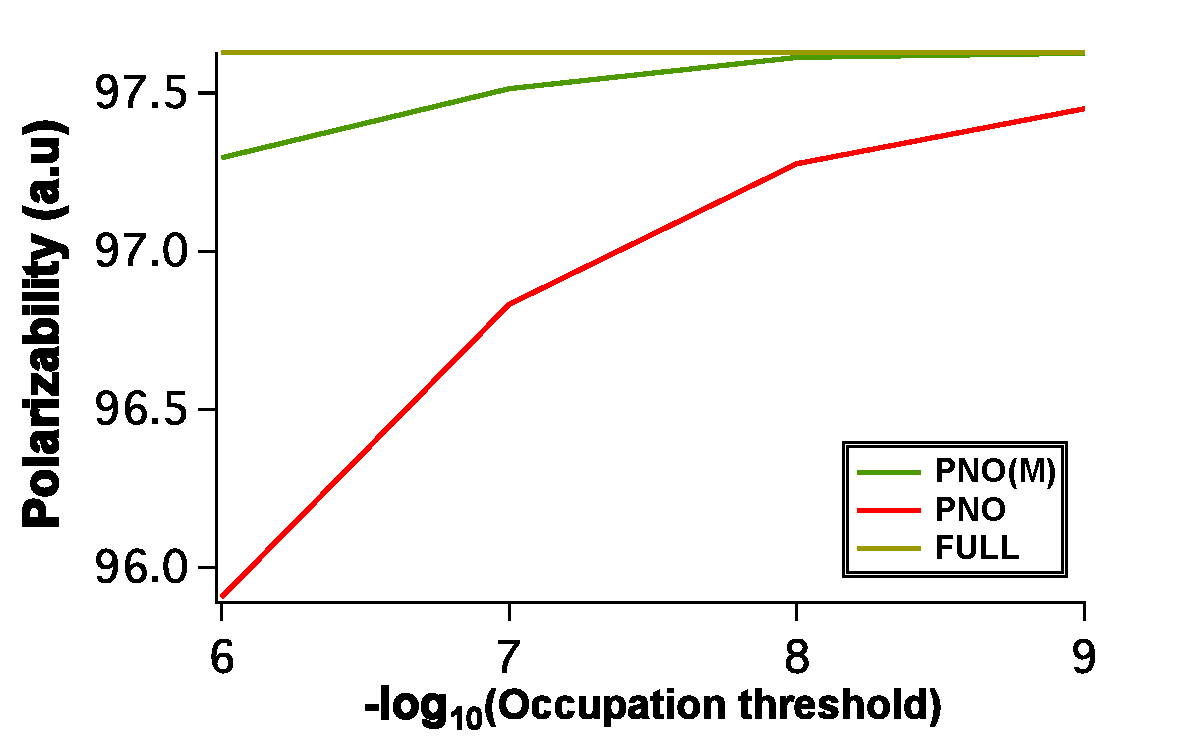
\includegraphics[width=0.6\linewidth,natwidth=610,natheight=642]{figures_pno++/pno_m_h2_7_adz_polar.pdf}
\caption{{\footnotesize CCSD/aDZ polarizabilities of (H$_2$)$_7$ in both PNO and PNO(M) approaches 
as a function of -log(occupation threshold).}}
\label{fig:pno_m_h2_7_polar}
\end{MyFigure}
compares the performance of both PNO(M) amd PNO approaches for calculating CCSD dynamic polarizabilities of
(H$_2$)$_7$ molecule at 589 nm. It can be seen that the PNO(M) scheme converges to the full result much 
faster than the PNO method. A cutoff of 10$^{-6}$ in the PNO(M) approach gives almost the same accuracy as 
a cutoff of 10$^{-9}$ for the PNO approach. Similar trends can be seen for specific rotation as well
for the same system (see Fig.~\ref{fig:pno_m_h2_7_optrot}),
\begin{MyFigure}[h!]
\centering
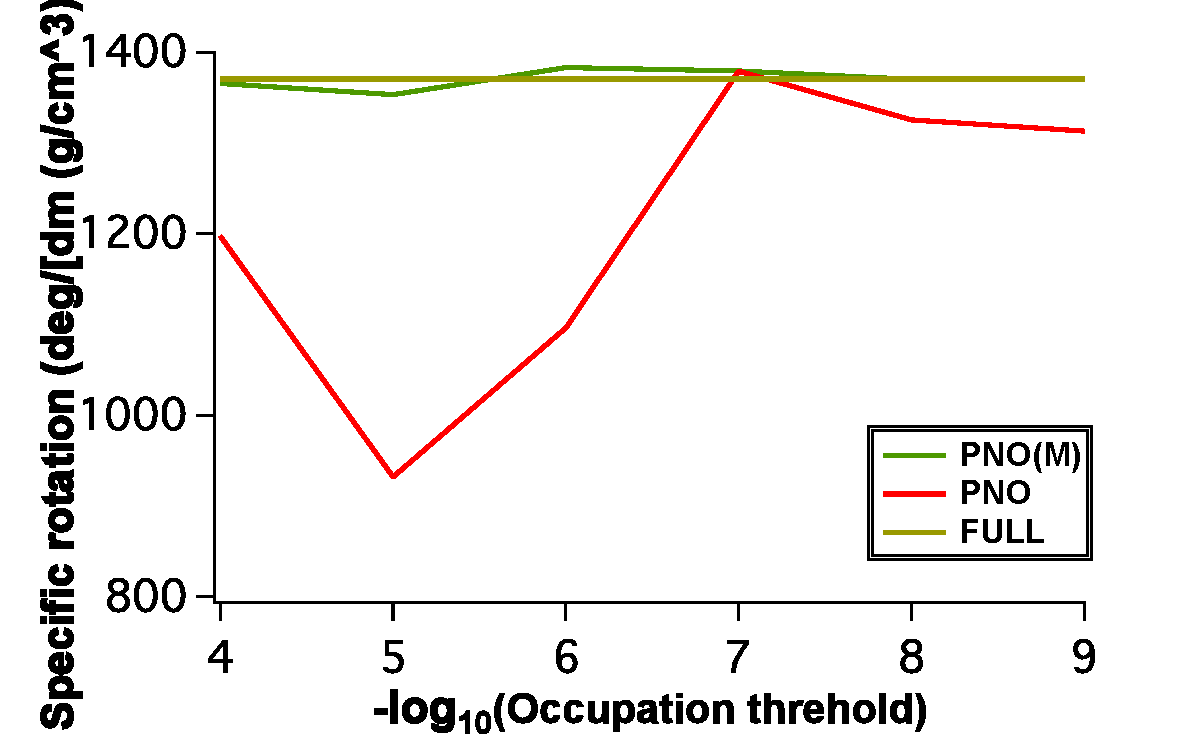
\includegraphics[width=0.6\linewidth,natwidth=610,natheight=642]{figures_pno++/pno_m_h2_7_adz_optrot.pdf}
\caption{{\footnotesize CCSD/aDZ/MVG Specific rotations of (H$_2$)$_7$ in both PNO and PNO(M) approaches
as a function of -log(occupation threshold)}}
\label{fig:pno_m_h2_7_optrot}
\end{MyFigure}
where even at a very high cutoff of 10$^{-4}$, the PNO(M) approach has almost converged to the full 
canonical result. On the other hand, the PNO approach even at a tight cutoff of 10$^{-9}$ doesn't
reproduce the canonical value. Furthermore, on account of fortuitous cancellation of errors in the
PNO approach, a cutoff of 10$^{-7}$ gives much more accurate results than 10$^{-9}$.
However, in the PNO(M) approach, evey pair of LMOs becomes ``important" as it always posesses 
a certain number of VMOs. Thus, the computational expenses are significantly higher in such an
approach. Also, the selection of the diffuse space is not straightforward as the criteria of 
spatial extents is not robust enough. We look at the PNO++($\mu$) approach to see if it can naturally
identify and retain the PNOs which are important for response properties.
Fig.~\ref{fig:pno_m_h2_4_polar_D}
\begin{MyFigure}[h!]
\centering
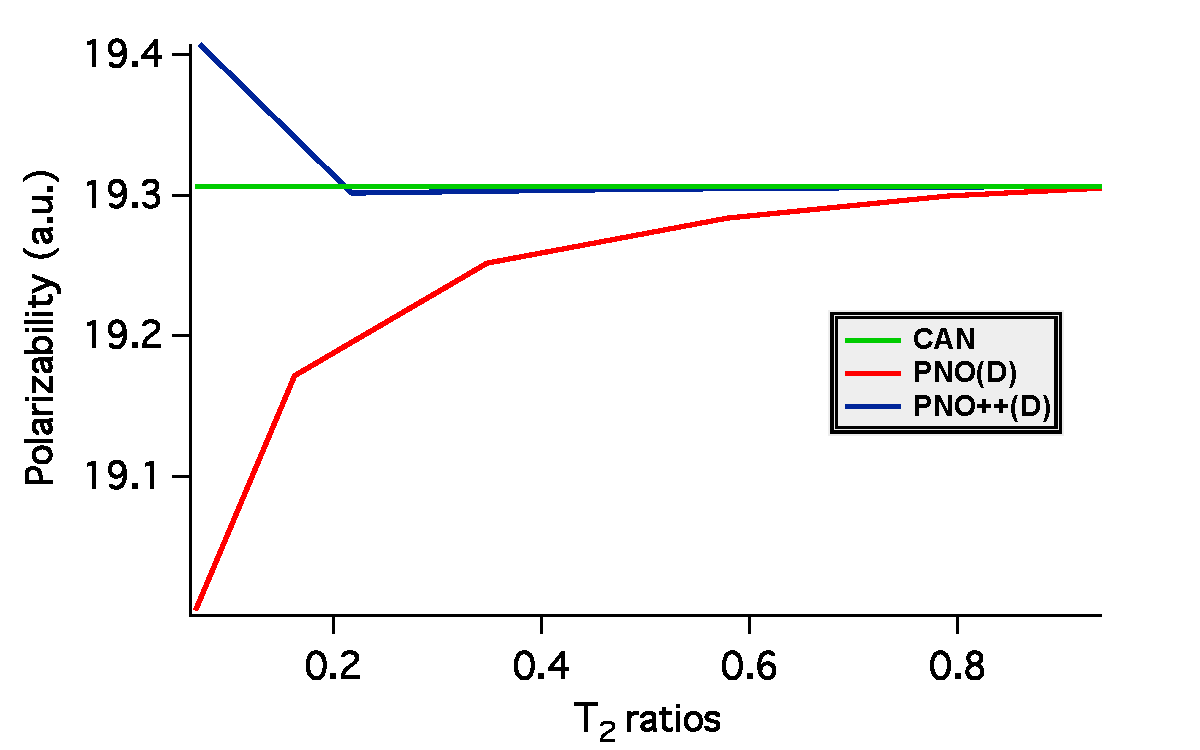
\includegraphics[width=0.6\linewidth,natwidth=610,natheight=642]{figures_pno++/h2_4_polar_D.pdf}
\caption{{\footnotesize CCSD/aDZ dynamic polarizabilities of (H$_2$)$_4$ at 589 nm in both PNO and PNO++($\mu$) approaches
with only doubles amplitudes truncated, as a function of T$_2$ ratios.}}
\label{fig:pno_m_h2_4_polar_D}
\end{MyFigure}
compares the performances of both PNO and PNO++($\mu$) approaches when the singles
amplitudes are kept untruncated in calculating CCSD dynamic polarizabilities 
of (H$_2$)$_4$. It can be easily seen that the PNO++ scheme significanty outperforms 
the PNO scheme and converges to the full result at a T2 ratio slightly greater 
than 0.2, while the PNO approach converges to the canonical result only after the retention
of more than 70\% of the doubles amplitudes. When both singles and doubles amplitudes
are truncated (see Fig.~\ref{fig:pno_m_h2_4_polar_SD}), the truncation errors increase
as expected, but the difference between the two approaches become more pronounced.
For example, the error in the PNO approach at a T2 ratio of 0.2 is an order of
magnitude greater than that of PNO++. 
\begin{MyFigure}[h!]
\centering
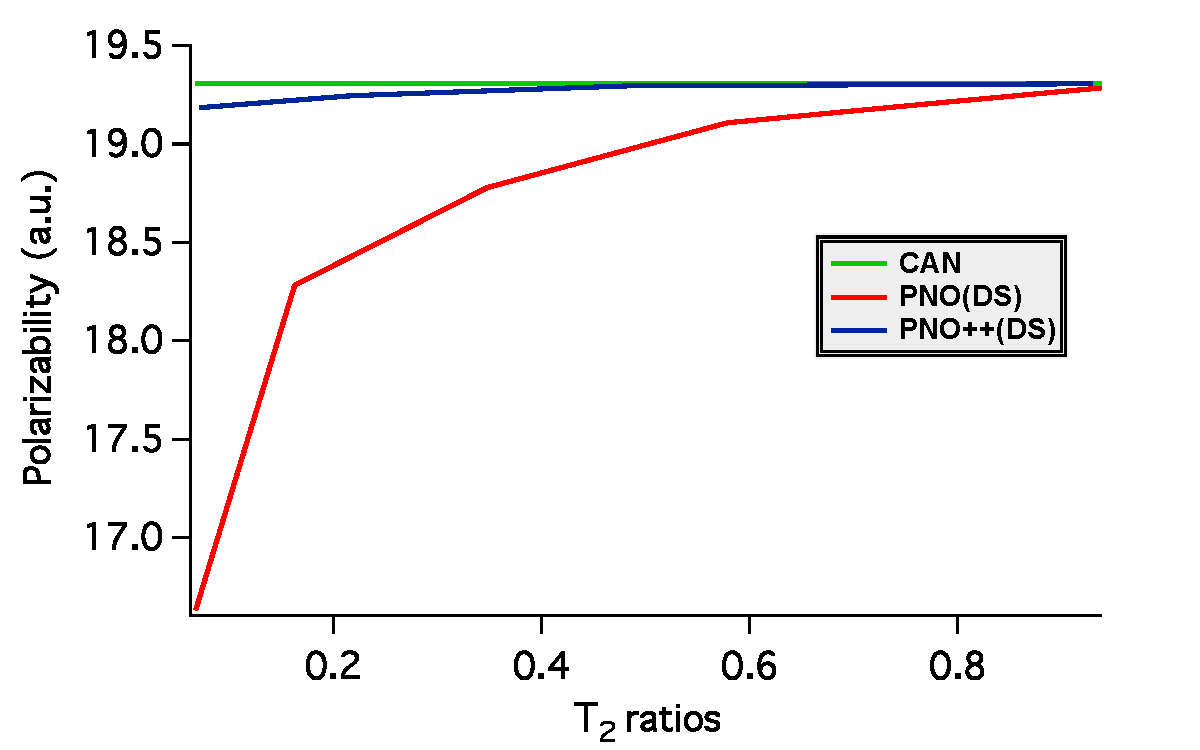
\includegraphics[width=0.6\linewidth,natwidth=610,natheight=642]{figures_pno++/h2_4_polar_DS.pdf}
\caption{{\footnotesize CCSD/aDZ polarizabilities of (H$_2$)$_4$ in both PNO and PNO++ approaches
with both singles and doubles amplitudes truncated, as a function of T$_2$ ratios.}}
\label{fig:pno_m_h2_4_polar_SD}
\end{MyFigure}
In a similar analysis for specific rotations, (see Fig.~\ref{fig:pno_m_h2_4_optrot_D})
\begin{MyFigure}[h!]
\centering
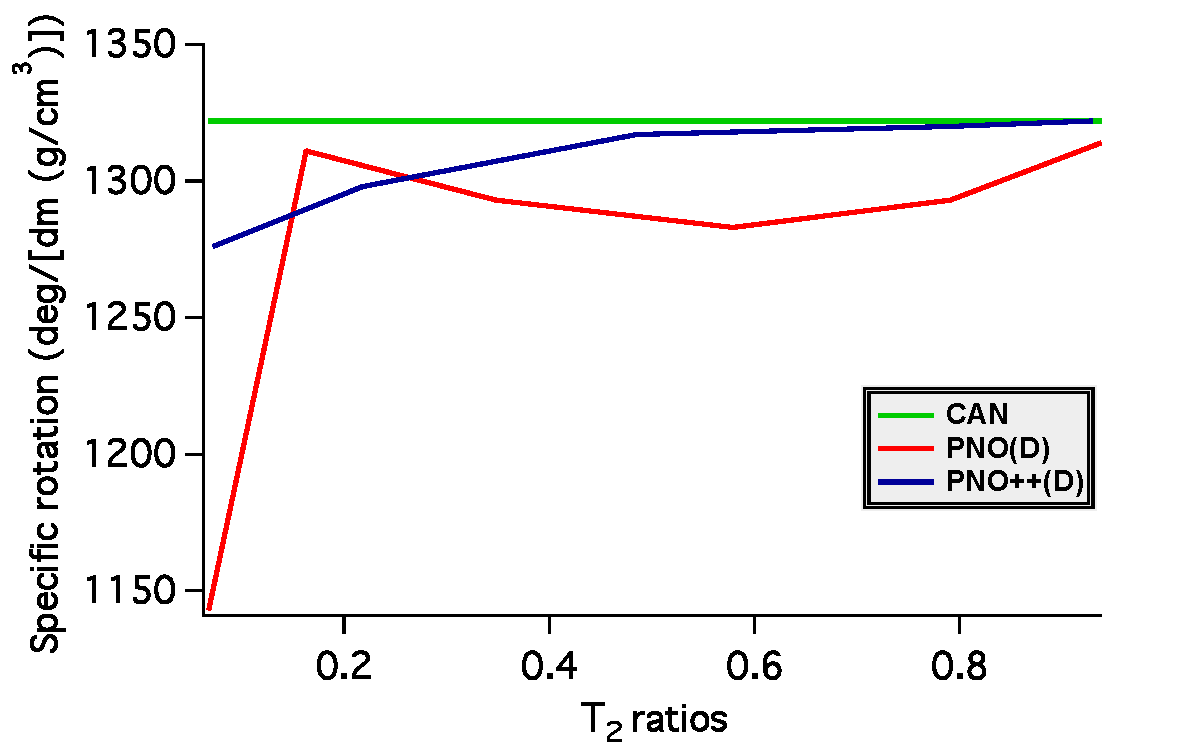
\includegraphics[width=0.6\linewidth,natwidth=610,natheight=642]{figures_pno++/h2_4_optrot_lg_D.pdf}
\caption{{\footnotesize CCSD/aDZ/LG specific rotations of (H$_2$)$_4$ in both PNO and PNO++ approaches
with only doubles amplitudes truncated, as a function of T$_2$ ratios.}}
\label{fig:pno_m_h2_4_optrot_D}
\end{MyFigure}
it can be seen that the truncation errors are higher compared to polarizabilities, which is not 
unexpected since specific rotations are found to be more sensitive to the wavefunction truncation.
When only doubles amplitudes are truncated, the specific rotations in the case of PNOs, continue 
to move farther away from the full result up to T2 ratios close to 0.6. Thereafter, it slowly 
converges towards the canonical result. On the other hand, the PNO++ curve has the right
convergence behavior: as the values of T2 ratios increase, it converges faster to the full result.
On truncating both singles and doubles amplitudes, (see Fig.~\ref{fig:pno_m_h2_4_optrot_SD})
\begin{MyFigure}[h!]
\centering
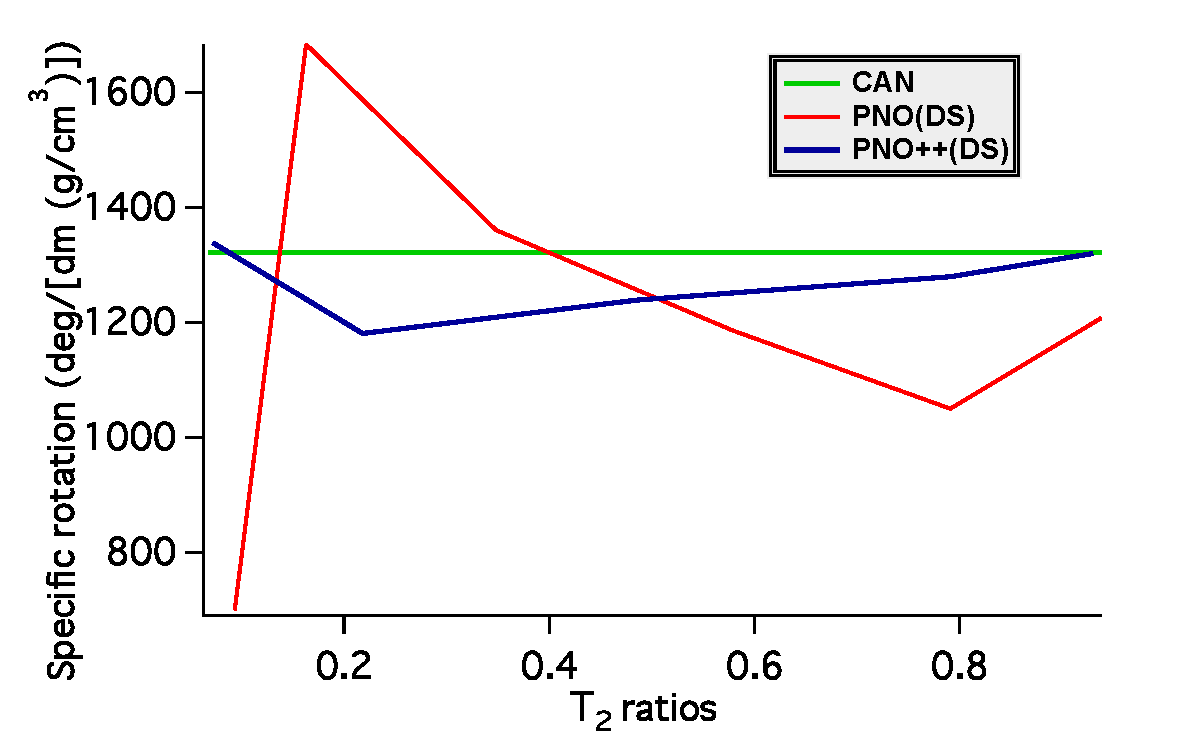
\includegraphics[width=0.6\linewidth,natwidth=610,natheight=642]{figures_pno++/h2_4_optrot_lg_DS.pdf}
\caption{{\footnotesize CCSD/aDZ/LG specific rotations of (H$_2$)$_4$ in both PNO and PNO++ approaches
with both singles and doubles amplitudes truncated, as a function of T$_2$ ratios.}}
\label{fig:pno_m_h2_4_optrot_SD}
\end{MyFigure}
the errors are much higher. The PNO curve starts moving towards the canonical result only 
after T2 ratios higher than 0.8 is achieved whereas the PNO++ graph starts converging
in the right direction after just 20\% of the wavefunction is retained.
%\subsection{$(H_2)_n$ Helices}
%First thing would be showing the retention of diffuse space. show the two graphs
%showing for (h2)7 systems. name it PNO(M) for modified PNO, mention that
%this is not feasible as big number of diffuse-functions, plus not a blackbox 
%way for selecting the cutoff for retention.
%- Linear structure, chiral, helical arrangement
%- best case for local correlation problems
%- small masses, high OR
%- Polariz, specific rotation (h2)4, (h2)5, (h2)6, (h2)7, maybe-bigger!! : LG, MVG, aDZ basis
%- diagnostics for FVNO++ approach:
%    - first comparing the structure of the ground state and perturbed density, one can see
%      that perturbed density would have a higher rank than ground-state density.
%    - how about incorporating L*L density as well and optimized NOs by better guess densities.
%    - Here we mostly concentrate on capturing the right kind of behavior rather
%    than savings, since there is not enough sparsity on offer for these cases.
%    This is applicable for other test cases as well.
%\subsection{beta-pinene}
%\subsection{phenyl-ethanol}
%\subsection{norbornenone}
%\pagebreak
\section{Conclusions}
We have a developed an extension of the PNO method, the PNO++ 
approach for calculating response properties. The pair 
specific densities constructed in this approach strongly
resemble in structure with the underlying response equations
and preliminary results on linear chain hydrogen helices
seem to indicate that the ONs obtained by diagonalizing these densities
are a good metric for estimating the importance of a
VNO in the response of the wavefunction. we plan to use this
method with RI-CC2/CCSD linear response theory to calculate  
CC level properties of large solvated clusters.
Furthermore, calculations on two and three dimensional structures 
involving different forms of second-order perturbed density 
are still running and are expected to give more insight
which can be used to make PNO++ a truly black-box method.



%The most popular approaches
%of inducing sparsity in the virtual orbital space 
%are based on the concept of Natural
%orbitals (NOs), introduced by L{\"o}wdin in 1955\cite{}as the eigenvectors of  
%the one electron reduced density matrices (1-RDMs), where he referred to 
%the corresponding eigenvalues as occupation numbers (ONs). L{\"o}wdin showed  
%the configuration interaction (CI) wavefunction expansion in the NO basis 
%converges quite rapidly compared to the CMO basis. Motivated by L{\"o}wdin's 
%findings, Bender, Barr and Davidson\cite{} used NOs obtained from 
%a few years later used approximate NOs 
%to construct optimized configurations in their CI calculations on first-row diatomic 
%hydrides. A Barr 
%and Davidson\cite{} employed what they called the frozen form of NOs 
%obtained by diagonalizing only the virtual-virtual block of the density 
%matrix to analyze the nature of the CI method through correlation energy 
%studies on Ne atom; Edminston and Krauss,\cite{}Meyer\cite{}, Ahlrichs and 
%co-workers\cite{} developed the concept of pair natural orbitals (PNOs) or 
%``pseudonatural orbitals" as the eigenvectors of the 1-RDM associated 
%with a single electron pair. 
%The ONs can be seen as a metric for estimating the importance of a virtual NO in describing
%electron correlation effects and hence all those virtual NOs which have ONs below a given threshold
%can be removed without causing any significant errors in correlation energies. 

%f. Recent work of FVNO and then PNO for excitation energies
%g. How about response properties?
%h. Properties are tough, cite all our papers, harley's paper, 
%Extension of harley's work, can the results be improved by making use of perturbed densities
%, cite my FVNO++ paper and explain the logic behind that
%  but that's only a reduced-prefactor method! how to make it reduced-scaling?
%i. Here we compare the performance of this approach for dynamic polarizabilities and specific 
